\chapter{Method} \label{cha:method}

This chapter presents the methodological foundations and concrete design of the
Robust Trinity, a multi-agent architecture for adversarially robust financial
trading. It first establishes the research strategy and justifies the choice of
a simulation-based experimental approach over alternatives such as formal
verification or field deployment (Section~\ref{sec:research_strategy}). The data
collection and analysis methods are then described
(Sections~\ref{sec:data_collection}--\ref{sec:data_analysis}), followed by a
discussion of alternative methods considered and the ethical implications of the
work (Sections~\ref{sec:alternatives}--\ref{sec:ethics}).
The chapter concludes with a detailed method application
(Section~\ref{sec:method-application}), which specifies the system architecture,
agent designs, evaluation protocol, and software tooling used throughout the
experimental work.


%--------------------------------------------------------------
\section{Research Strategy} \label{sec:research_strategy}
%--------------------------------------------------------------

Research strategies are high-level plans that govern the research process~\cite{johannesson2014design}---for example, experiments, case studies, surveys,
and action research. Each strategy is accompanied by particular research methods
used primarily for data collection and analysis. This section identifies and
justifies the strategy adopted in this thesis.

This thesis follows a \textit{design science research} (DSR) strategy, as it
centres on the development and evaluation of an artifact---the Robust Trinity
architecture---intended to solve a practical problem in adversarial financial
decision-making. Design science research is a research strategy in which
knowledge is generated through the design and evaluation of artifacts that
address identified problems~\cite{johannesson2014design, articlehevner}. This
aligns with the thesis's objective: to design a multi-agent system that produces
safe and economically viable trading actions under adversarial conditions.

We operationalise this strategy using the five-activity process model proposed
by~\cite{johannesson2014design}: \textit{Explicate Problem}, \textit{Define
Requirements}, \textit{Design and Develop Artifact}, \textit{Demonstrate
Artifact}, and \textit{Evaluate Artifact}. Following the research question's
focus on the performance and robustness of the proposed architecture, the
framework is applied with emphasis on the development and evaluation activities,
which are approached more rigorously than the others. Each activity employs
distinct research strategies and methods, outlined below.

\begin{description}
    \item[Explicate Problem.] The research strategy used in this activity is a
    \textit{literature survey and synthesis}. Existing work on adversarial
    machine learning, multi-agent financial systems, and robust aggregation
    mechanisms is surveyed and synthesised to identify the specific gap that
    motivates the artifact: the absence of inference-time, cross-modal
    arbitration in heterogeneous financial AI
    (Chapters~\ref{cha:extendBackground}).

    \item[Define Requirements.] The method applied is \textit{analytical
    derivation} from the research questions. The main research question and its
    sub-questions are translated into concrete architectural requirements---channel
    independence between the semantic and numeric reasoning paths, cross-modal
    consistency detection via a divergence metric, and fail-safe default
    behaviour under high disagreement---that the artifact must satisfy.

    \item[Design and Develop Artifact.] The research strategy is
    \textit{constructive}: the architecture is designed as a composition of three
    heterogeneous agents---an LLM-based semantic analyst, an RL-based numeric
    executor, and a rule-based risk guardian---each operating on a distinct
    modality and coordinated through a divergence-based arbitration mechanism
    (the C-Gate). Design decisions are justified by the requirements
    derived in the preceding activity. This activity encompasses data collection
    and preprocessing (Section~\ref{sec:data_collection}), agent training
    (Section~\ref{sec:executor}), LLM signal generation
    (Section~\ref{sec:analyst}), and calibration of the arbitration mechanism
    (Section~\ref{sec:cgate}).

    \item[Demonstrate Artifact.] The strategy is a \textit{simulation-based case
    study}. The system is instantiated on historical equity market data for a
    single ticker (AAPL) and executed under nominal, non-adversarial conditions
    to verify that it produces functionally correct trading behaviour---that the
    three-regime decision policy activates as intended and that the Guardian's
    risk constraints are respected---before adversarial evaluation.

    \item[Evaluate Artifact.] The strategy is a \textit{controlled experiment},
    characterised by systematic manipulation of independent variables and
    observation of dependent outcomes~\cite{denscombe2017good}. Two adversarial
    attack types are applied at controlled intensity levels to isolated system
    channels: analyst signal poisoning (flipping directional recommendations at
    five corruption rates) and executor observation perturbation (adding Gaussian
    noise at five standard deviation levels). Robustness is assessed through
    financial risk metrics---Sharpe ratio, maximum drawdown (MaxDD), Sortino
    ratio---against four baseline system configurations. This activity
    constitutes the primary empirical contribution of the thesis.
\end{description}

The described approach aligns with established practices in the applied machine
learning literature. Studies in adversarial robustness and multi-agent
financial AI typically identify a gap in the literature (Explicate Problem),
propose an architecture or method (Design and Develop), and evaluate it through
controlled experiments against baselines
(Evaluate)~\cite{benhenda2025finrl, xia_bayesian_2026, baviskar2025robust}.
This thesis follows the same pattern, with the addition of the DSR process
model to structure the work explicitly.


%--------------------------------------------------------------
\section{Data Collection Methods} \label{sec:data_collection}
%--------------------------------------------------------------

Data collection in this study follows three streams, corresponding to the inputs
required by the Executor (numeric market features), the Analyst (financial news
headlines), and the C-Gate (precomputed LLM signals). All data is collected as
secondary data from publicly available sources~\cite{denscombe2017good}, and no
primary data involving human participants is generated.

%--------------------------------------------------------------
\subsection{Historical Market Data} \label{sec:market_data}
%--------------------------------------------------------------

Daily open-high-low-close-volume (OHLCV) data for Apple~Inc. (AAPL) is
obtained from Yahoo Finance via the \texttt{yfinance} Python library, with
automatic split and dividend adjustment enabled. The download period spans
1~July~2018 to 31~December~2024; the start date is set approximately 252
trading days before the intended training start of 1~January~2020 to provide a
warm-up window for the rolling normalisation described in
Section~\ref{sec:feature_engineering}. The raw OHLCV data is stored in Apache
Parquet format. A single global seed of~42 is set before download to ensure
deterministic behaviour in any stochastic library operations.

Figure~\ref{fig:aapl_data} illustrates the evolution of AAPL closing prices
and trading volume over the study period, along with the chronological split
points used in the experimental setup.

\begin{figure}[h]
    \centering
    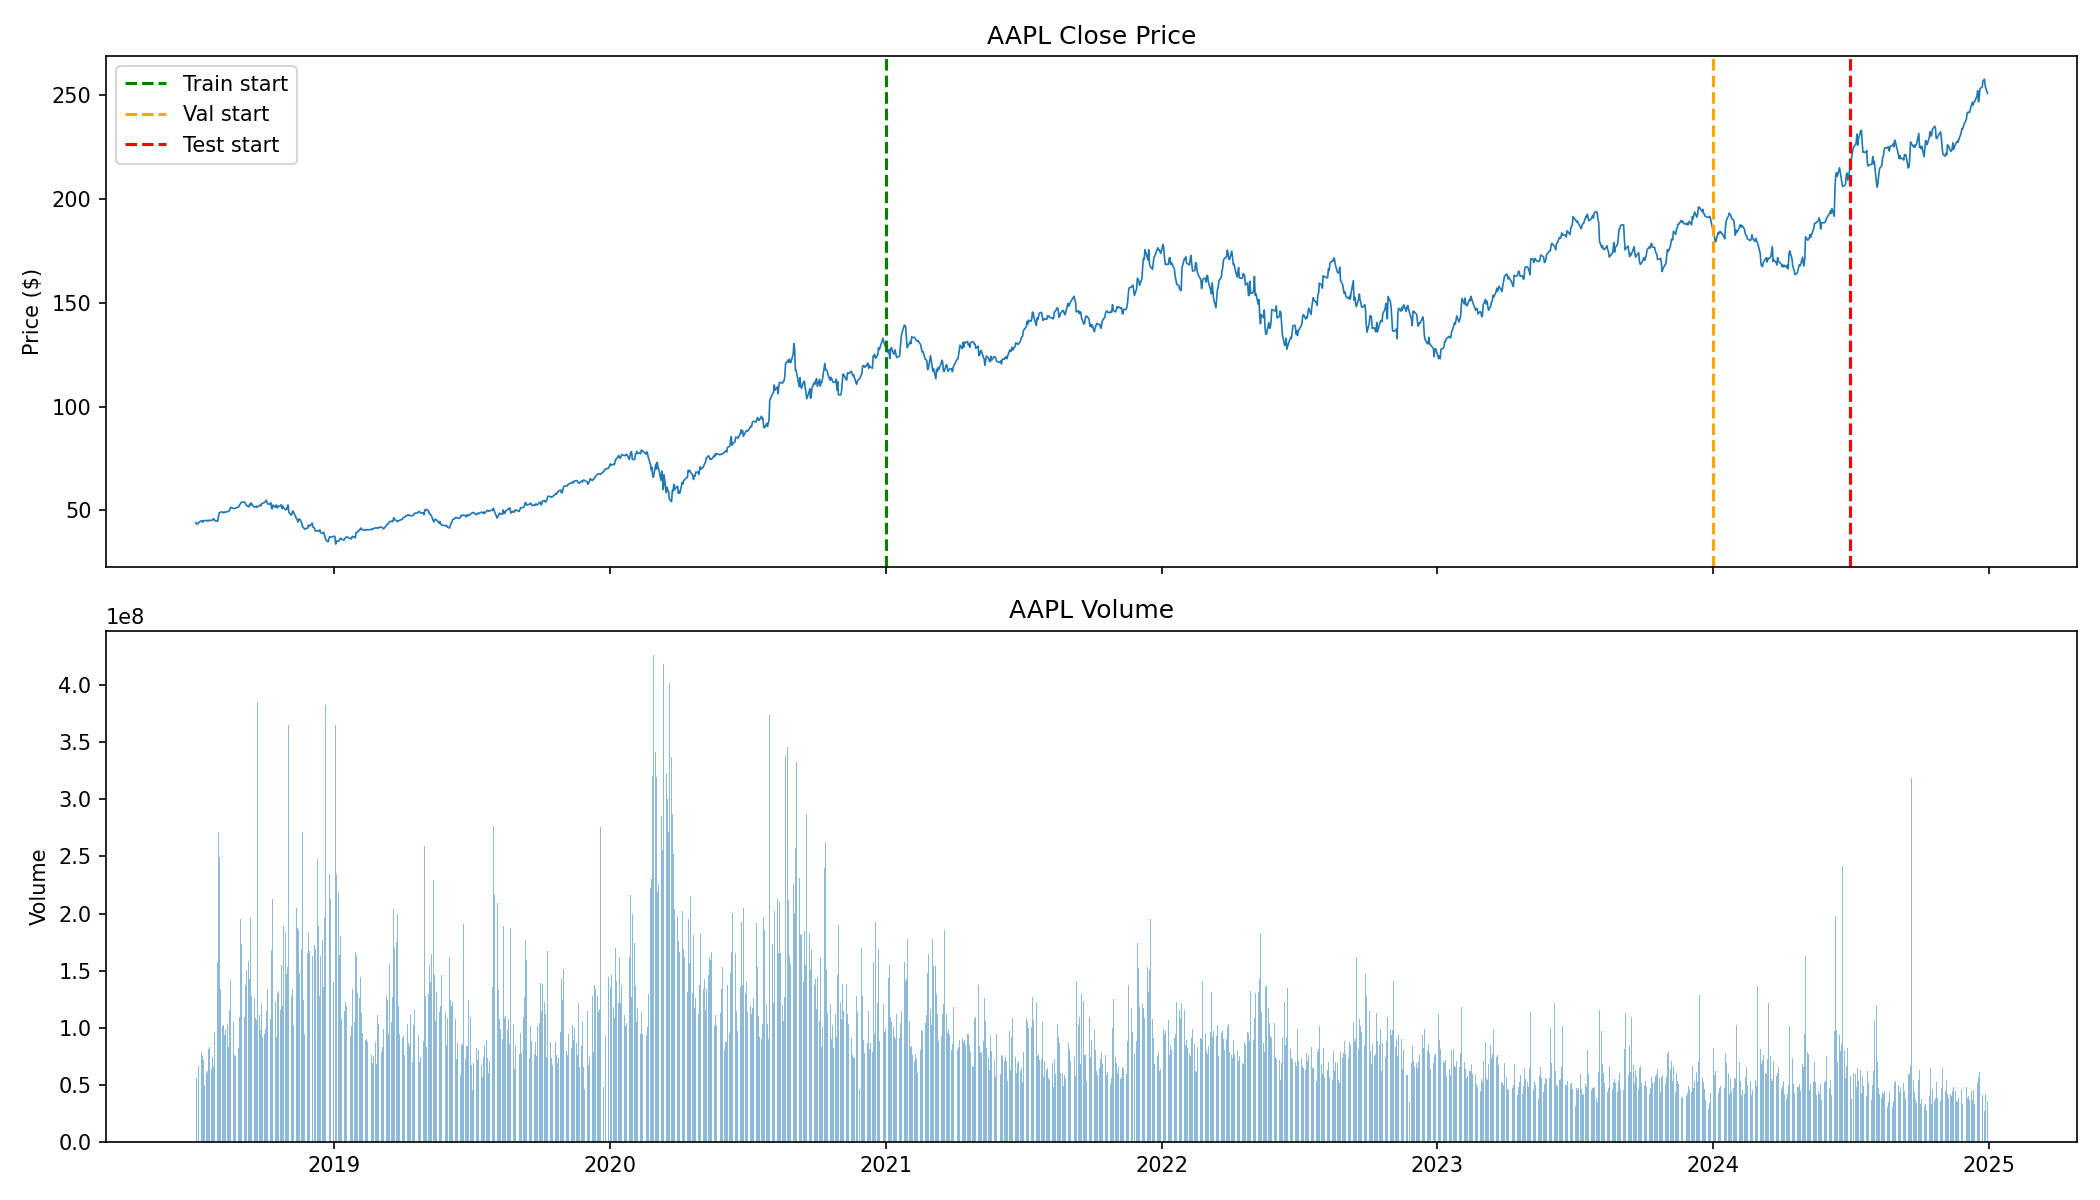
\includegraphics[width=\linewidth]{price_and_volume.png}
    \caption{AAPL closing price (top) and trading volume (bottom) from 2018 to 2024.
    The green dashed line indicates the start of the training period, yellow indicates start of validation period, while the red
    dashed line marks the beginning of the test period.}
    \label{fig:aapl_data}
\end{figure}
The data is partitioned into four chronological, non-overlapping splits.
Table~\ref{tab:data_splits} summarises the split boundaries.

\begin{table}[h]
\centering
\caption{Chronological data splits. All dates are inclusive.}
\label{tab:data_splits}
\begin{tabular}{@{}llll@{}}
\toprule
\textbf{Split} & \textbf{Start} & \textbf{End} & \textbf{Purpose} \\
\midrule
Warm-up  & 2020-01-01 & 2020-12-31 & Rolling normalisation warm-up; not used for training \\
Train    & 2021-01-01 & 2023-12-31 & PPO policy training ($\approx$750 trading days) \\
Val      & 2024-01-01 & 2024-06-30 & Early stopping, hyperparameter selection, C-Gate calibration \\
Test     & 2024-07-01 & 2024-12-31 & Held-out evaluation ($\approx$126 trading days) \\
\bottomrule
\end{tabular}
\end{table}

The choice of a single equity (AAPL) is a deliberate delimitation. It reduces
confounding factors arising from cross-asset correlation and sector-specific
dynamics, allowing the evaluation to isolate the effect of the architectural
design. The codebase is designed to be ticker-agnostic---all data loading,
feature engineering, and training functions accept a ticker parameter---and
multi-asset extension is discussed as future work.

\subsubsection{Feature Engineering} \label{sec:feature_engineering}

From the raw OHLCV data, 14 technical features are computed. These features
capture price momentum, volatility, volume dynamics, and intraday range, and
are chosen to provide the Executor with a diverse but standard set of market
signals. Table~\ref{tab:features} lists each feature, its computation, and the
relevant parameters.

\begin{table}[h]
\centering
\caption{Technical features derived from OHLCV data.}
\label{tab:features}
\begin{tabular}{@{}rllp{5cm}@{}}
\toprule
\textbf{\#} & \textbf{Feature} & \textbf{Parameters} & \textbf{Computation} \\
\midrule
1  & \texttt{log\_return}       & ---               & $\log(C_t / C_{t-1})$ \\
2  & \texttt{rsi}               & period = 14       & Relative Strength Index (Wilder's EMA) \\
3  & \texttt{macd\_line}        & fast=12, slow=26  & $\text{EMA}(C, 12) - \text{EMA}(C, 26)$ \\
4  & \texttt{macd\_signal}      & signal = 9        & $\text{EMA}(\text{MACD}, 9)$ \\
5  & \texttt{macd\_histogram}   & ---               & MACD line $-$ signal \\
6  & \texttt{bb\_upper}         & period=20, $k$=2  & $\text{SMA}(C, 20) + 2 \cdot \text{STD}(C, 20)$ \\
7  & \texttt{bb\_lower}         & period=20, $k$=2  & $\text{SMA}(C, 20) - 2 \cdot \text{STD}(C, 20)$ \\
8  & \texttt{bb\_percent\_b}    & period=20, $k$=2  & $(C - \text{lower}) / (\text{upper} - \text{lower})$ \\
9  & \texttt{atr}               & period = 14       & EMA of True Range \\
10 & \texttt{volume\_ratio}     & period = 20       & $V_t / \text{SMA}(V, 20)$ \\
11 & \texttt{realized\_vol}     & window = 20       & Rolling std of log returns \\
12 & \texttt{close}             & ---               & Raw close price (normalised subsequently) \\
13 & \texttt{high\_low\_range}  & ---               & $(H_t - L_t) / C_t$ \\
14 & \texttt{close\_open\_return} & ---             & $(C_t - O_t) / O_t$ \\
\bottomrule
\end{tabular}
\end{table}

All 14 features are then normalised using a rolling z-score with a 252-day
window (approximately one trading year). For each feature $x$ at time $t$:
\begin{equation}
z_t = \frac{x_t - \bar{x}_{t-252:t}}{\sigma_{t-252:t}},
\end{equation}
where $\bar{x}$ and $\sigma$ denote the rolling mean and standard deviation
over the preceding 252 trading days. A minimum of 20 observations is required
before z-scores are computed; earlier rows are dropped. Standard deviations
below $10^{-8}$ are replaced with $10^{-8}$ to avoid division by zero.

Rolling normalisation is preferred over global normalisation because it avoids
information leakage from future data into earlier observations and because it
adapts to non-stationary market dynamics. The 252-day window captures
approximately one calendar year of trading activity, providing stable estimates
while remaining responsive to regime shifts.

An automated channel-independence check verifies that no feature column name
contains keywords associated with text-derived data (e.g., \texttt{sentiment},
\texttt{headline}, \texttt{embedding}). This programmatic assertion enforces
the design requirement that the Executor operates exclusively on numeric market
signals, with no access to any information derived from the Analyst's textual
inputs.

%--------------------------------------------------------------
\subsection{Financial News Headlines} \label{sec:headlines}
%--------------------------------------------------------------

Financial news headlines for AAPL are collected via the Polygon.io REST API
(\texttt{/v2/reference/news}), using a free-tier API key. The query spans
1~January~2020 to 31~December~2024 and is filtered to articles that list AAPL
in their \texttt{tickers} field. Pagination follows Polygon's cursor-based
\texttt{next\_url} mechanism with a rate limit of 5~requests per minute (12.5
seconds between requests).

The raw article set is deduplicated to yield exactly one headline per trading
day. Non-trading days (weekends and market holidays) are identified by
cross-referencing the headline dates against the dates present in the OHLCV
data; headlines falling on non-trading days are discarded. When multiple
articles exist for a single trading day, the first article by
\texttt{published\_utc} ascending is retained. This deduplication ensures a
one-to-one mapping between trading days and Analyst inputs.

The resulting dataset contains 1{,}021 headlines spanning 15~April~2020 to
27~December~2024. The six most frequent sources are Benzinga (312 headlines),
The Motley Fool (225), Zacks Investment Research (135), MarketWatch (131),
Seeking Alpha (120), and Investing.com (80). Coverage is approximately 81\% of
trading days in the full period. Days without a headline are handled as missing
Analyst signals during integration (see Section~\ref{sec:cgate}).

Each headline entry is stored as a JSON object with four fields:
\texttt{date} (ISO~8601 format), \texttt{ticker}, \texttt{headline} (article
title), and \texttt{source} (publisher name).

%--------------------------------------------------------------
\subsection{LLM Signal Generation} \label{sec:signal_generation}
%--------------------------------------------------------------

For each of the 1{,}021 headlines, a trading signal is generated by submitting
the headline to GPT-5 (accessed via Azure OpenAI, deployment
\texttt{gpt-5-chat}) with a temperature of~0.0 (greedy decoding) and a maximum
token limit of~1{,}024. The model is instructed to respond in JSON format using
the structured output mode provided by the Azure OpenAI API.

\subsubsection{Prompt Design}

The system prompt assigns the model the role of a ``highly decisive quantitative
financial analyst'' and imposes the following constraints:

\begin{enumerate}
    \item \textbf{Reasoning first.} The model must write its chain-of-thought
    reasoning \textit{before} committing to a decision. This ordering is
    enforced structurally: the \texttt{reasoning} field precedes the
    \texttt{decision} field in the JSON schema, preventing premature commitment.
    \item \textbf{Directional bias.} Any headline containing material positive
    or negative sentiment must be classified as \texttt{buy} or \texttt{sell},
    respectively. The prompt explicitly states: ``hold is strictly for perfectly
    neutral or irrelevant headlines.''
    \item \textbf{No hedging.} The model is instructed not to hedge with
    \texttt{hold} when directional evidence exists.
    \item \textbf{No numeric data.} The model must base its decision solely on
    the headline text, without referencing any market data.
\end{enumerate}

Five few-shot examples are included in the system prompt to calibrate the
model's decision boundaries:

\begin{enumerate}
    \item Apple Q3 earnings beat expectations $\rightarrow$ \textbf{buy} (AAPL)
    \item FDA rejects Pfizer drug application $\rightarrow$ \textbf{sell} (PFE)
    \item Tesla regional charging partnership $\rightarrow$ \textbf{hold} (TSLA)
    \item Microsoft antitrust investigation $\rightarrow$ \textbf{sell} (MSFT)
    \item Amazon AWS brief outage $\rightarrow$ \textbf{hold} (AMZN)
\end{enumerate}

These examples are drawn from multiple tickers to encourage generalisation
rather than overfitting to AAPL-specific patterns.

\subsubsection{Output Schema}

The model's output is validated against a Pydantic schema with two fields:

\begin{itemize}
    \item \texttt{reasoning} (\texttt{str}): chain-of-thought analysis of the
    headline's implications. Must not be empty.
    \item \texttt{decision} (\texttt{Literal["hold", "buy", "sell"]}): the
    directional trading recommendation.
\end{itemize}

Critically, the Analyst does \textit{not} produce a confidence score. The
decision is categorical---one of three discrete values---and the reasoning
trace serves as an interpretability artifact rather than a quantitative input to
the C-Gate. This design simplifies the divergence metric
(Section~\ref{sec:cgate}) and avoids the calibration challenges associated with
LLM-generated confidence estimates.

\subsubsection{Precomputation and Caching}

All 1{,}021 signals are precomputed offline and cached in a JSON file. Each
entry is keyed by a SHA-256 hash of the concatenation
\texttt{ticker|date|headline}, truncated to 16~hexadecimal characters. The
precomputation pipeline is resumable: on restart, it loads the existing cache
and skips already-computed entries. A checkpoint is written every 10~new
computations, with atomic file writes (write to a temporary file, then rename)
to prevent corruption on interruption. The inter-call delay is 0.3~seconds to
remain within API rate limits.

The final signal distribution across the 1{,}021 headlines is: \texttt{hold}
612 (59.9\%), \texttt{buy} 228 (22.3\%), \texttt{sell} 181 (17.7\%). The 40.1\%
directional rate (buy or sell) reflects the prompt's emphasis on decisiveness
and is substantially higher than the 9.7\% directional rate produced by a
smaller model (Llama~3.1~8B) under the same prompt, which was rejected due to
excessive passivity. Up to three retries with linear backoff are attempted per
headline; if all fail, a neutral fallback signal (\texttt{hold}) is recorded.


%--------------------------------------------------------------
\section{Data Analysis Methods} \label{sec:data_analysis}
%--------------------------------------------------------------

Data analysis proceeds through quantitative methods applied to the trading
outputs produced by each system configuration. Three categories of analysis are
conducted: financial performance measurement, robustness assessment under
adversarial conditions, and systematic ablation.

%--------------------------------------------------------------
\subsection{Financial Performance Metrics} \label{sec:financial_metrics}
%--------------------------------------------------------------

Each evaluation run produces a sequence of daily portfolio returns
$\{r_t\}_{t=1}^{T}$ from which four standard metrics---Sharpe ratio,
Sortino ratio, MaxDD, and total return---are computed as
defined in Section~\ref{sec:perf-metrics-bg}. Two implementation choices
are worth noting: the Sharpe ratio uses the population standard deviation
($\text{ddof} = 0$) rather than the sample standard deviation, and the
Sortino ratio uses a target return of zero. Among these four metrics, MaxDD
serves as the \emph{primary robustness indicator} in this thesis: a system
that limits drawdown under adversarial stress demonstrates architectural
fault containment even if its expected return is not positive.

%--------------------------------------------------------------
\subsection{Robustness Analysis} \label{sec:robustness_analysis}
%--------------------------------------------------------------

Robustness is assessed by comparing each system configuration's financial
metrics under benign (non-adversarial) conditions against the same metrics under
two controlled adversarial attack types applied at multiple intensity levels.
The adversarial protocol is described in detail in
Section~\ref{sec:adversarial_protocol}.

The primary robustness measure is the \textit{stability of MaxDD
under attack}. For a given system configuration, if MaxDD remains bounded within a
narrow range as attack intensity increases---while baseline configurations
exhibit growing MaxDD---this constitutes evidence that the architecture contains
adversarial damage rather than propagating it. Secondary robustness measures
include changes in Sharpe ratio and Sortino ratio across attack intensities.

All metrics are computed per seed and then aggregated across the four frozen
seeds as mean $\pm$ standard deviation, providing a measure of variability
across policy initialisations.

%--------------------------------------------------------------
\subsection{Ablation Design} \label{sec:ablation_design}
%--------------------------------------------------------------

A systematic ablation study isolates the contribution of each architectural
component to overall performance and robustness. Five system configurations are
evaluated under identical data splits, market conditions, and adversarial
protocols:

\begin{enumerate}
    \item \textbf{Trinity} (full system): Executor + Analyst + C-Gate +
    Guardian. The proposed architecture with all components active.

    \item \textbf{Executor-Only}: The PPO policy executes
    $\text{argmax}(\pi_{\text{RL}})$ at full position size. No Analyst signals,
    no C-Gate, no Guardian. Isolates the RL agent's standalone performance.

    \item \textbf{Analyst-Only}: The GPT-5 signal is executed directly as a
    trading action at full position size. No RL, no C-Gate, no Guardian.
    Isolates the LLM's standalone trading quality. This configuration has no
    seed variation (the LLM signals are deterministic at temperature~0.0) and
    produces a single trajectory per split.

    \item \textbf{Trinity-no-CGate}: A naive agreement heuristic replaces the
    C-Gate. If $\text{argmax}(\pi_{\text{RL}}) = a_{\text{LLM}}$, execute at
    full position; otherwise, execute $\text{argmax}(\pi_{\text{RL}})$ at 50\%
    position. No divergence metric, no thresholds, no Guardian. Tests whether
    simple agreement checking provides comparable robustness to the
    divergence-based C-Gate.

    \item \textbf{Buy-and-Hold}: Passive long position in AAPL over the
    evaluation period. No model, no transaction costs. Provides an
    unconditional market baseline.
\end{enumerate}

Comparing Trinity against Executor-Only isolates the combined effect of the
Analyst, C-Gate, and Guardian. Comparing Trinity against Trinity-no-CGate
isolates the specific contribution of the divergence-based C-Gate over naive
agreement checking. Comparing Trinity against Analyst-Only verifies that the
architecture does not merely inherit the LLM's decisions but adds value through
cross-modal arbitration. The buy-and-hold baseline contextualises all results
against the underlying market trend during the evaluation period.

%--------------------------------------------------------------
\subsection{Statistical Methods} \label{sec:statistical_methods}
%--------------------------------------------------------------

Descriptive statistics---means, standard deviations, and per-seed
breakdowns---are used to summarise results across the four frozen seeds.
Given the small sample size ($n = 4$ seeds), formal inferential tests such as
paired $t$-tests or bootstrap confidence intervals have limited statistical
power and are not reported in the current evaluation. This is acknowledged as a
limitation; multi-asset expansion (providing additional independent evaluation
contexts) and bootstrap-based confidence intervals are identified as priorities
for future work.

Where individual seed results are reported alongside aggregated means, the
per-seed breakdown provides transparency about the variability of outcomes
across policy initialisations---a form of sensitivity analysis that, while not
a substitute for formal inference, reveals whether conclusions depend on a
single favourable seed or hold consistently.

\section{Alternative Research Strategies and Methods}
\label{sec:alternatives}

This section discusses the main methodological and technical alternatives that were considered during the design of this study and explains the rationale for the choices ultimately made.

\subsection{Research Strategy Alternatives}

The overarching research strategy of design science research was chosen for its alignment with the artefact-centric goal of this study (Section~\ref{sec:research_strategy}). Two alternatives were considered. First, a \emph{pure experimental} strategy---training several RL agent variants, measuring performance, and reporting results without framing the work as artefact design---would have been feasible for the Executor component in isolation. However, it would not naturally accommodate the iterative, multi-component design process through which the C-Gate and Guardian were developed; design science research provides an explicit vocabulary for that process. Second, a \emph{case study} strategy could have situated the Trinity system within a specific trading desk or fund context, but access to proprietary order-flow data or live execution infrastructure was not available, making a controlled laboratory study more appropriate.

\subsection{Data Collection Alternatives}

Three data-related alternatives were evaluated and ultimately set aside.

\paragraph{Multi-asset universe.}
The original study plan envisioned applying the system to Nasdaq-100 constituents rather than a single ticker. A multi-asset setup would have strengthened external validity by exposing the C-Gate to diverse volatility regimes and sector-specific news dynamics. However, training and evaluating four PPO seeds per ticker across 100 tickers, combined with the cost of precomputing LLM signals for each, exceeded the available computational budget. The study therefore restricts itself to AAPL daily bars and notes single-ticker scope as a delimitation (Section~\ref{sec:delimitations}).

\paragraph{Additional text sources.}
Social media feeds (Reddit, X) and corporate filings (10-K, 10-Q) were considered as supplementary inputs to the Analyst. Social media data would have introduced real-time sentiment but also noise, bot activity, and non-trivial deduplication challenges. Corporate filings would have added fundamental context but arrive at quarterly cadence, poorly matched to the daily decision frequency of the system. To keep the Analyst's input channel well-controlled, only Polygon.io news headlines were retained---a single, professionally curated source with daily coverage.

\paragraph{Synthetic market simulation.}
Agent-based market simulators such as ABIDES~\cite{10.1145/3384441.3395986} were considered for generating controlled adversarial market microstructure. A simulation environment would have enabled systematic variation of order-book dynamics, flash-crash scenarios, and liquidity shocks. However, the calibration effort required to produce realistic daily-bar price series from an agent-based simulator was judged disproportionate to its benefit for a study focused on signal-level robustness. The post-hoc adversarial protocol adopted instead---analyst signal poisoning and executor observation perturbation (Section~\ref{sec:robustness_analysis})---provides targeted, reproducible robustness tests without introducing the confound of simulator fidelity.

\subsection{Technical Design Alternatives}
\label{sec:technical-alternatives}

Several technical alternatives were explored during the iterative development of the artefact, each evaluated empirically before a final design was locked.

\paragraph{Divergence metric.}
An early design considered the Jensen--Shannon divergence (JSD) between a pseudo-distribution derived from the Analyst's output and the Executor's policy distribution. This would have required the Analyst to produce a confidence score alongside its directional decision, yielding a three-element vector that could be compared with $\pi_{\mathrm{RL}}$ via JSD. However, eliciting calibrated confidence estimates from large language models remains an open problem~\citep{kadavath2022language}; pilot experiments showed that GPT-5 confidence scores exhibited poor calibration and added a noisy dimension without improving regime discrimination. The adopted metric, $\Delta_t = 1 - \pi_{\mathrm{RL}}(d_{\mathrm{LLM}} \mid s_t)$, uses only the Executor's own probability for the Analyst's recommended action---an asymmetric measure that requires no additional Analyst output and is fully determined by information already available in the pipeline.

\paragraph{Reward function.}
The Executor was initially trained with the Differential Sharpe Ratio (DSR)~\cite{moody2001learning}, a risk-adjusted reward that penalises volatility at each timestep through an exponential moving average of return moments. While theoretically appealing---DSR directly optimises the quantity the system is ultimately evaluated on---the per-step signal proved too weak for PPO to learn differentiated policies on a dataset of 756 trading days. Replacing DSR with a stateless log-return reward, $r_t = \log(1 + R_t^{\mathrm{portfolio}})$, resolved this issue and was adopted for all frozen models. The training progression and diagnostic criteria that informed this decision are detailed in Section~\ref{sec:seed-selection}.

\paragraph{Temperature scaling.}
Temperature scaling modulates the sharpness of the softmax distribution used to compute $\Delta_t$. A sweep over $T \in \{0.01, 0.02, 0.05, 0.1, 0.2\}$ initially identified $T = 0.05$ as the best setting by mean validation Sharpe. However, post-hoc inspection revealed that low temperatures collapsed the $\Delta$ distribution to bimodal values $\{0, 1\}$, producing degenerate thresholds that eliminated the Conflict regime entirely. Setting $T = 1.0$---i.e., using the raw policy probabilities without any rescaling---restored a continuous $\Delta$ distribution with well-separated thresholds and a healthy three-regime split. Temperature was accordingly fixed at $T = 1.0$ for all reported results.

\paragraph{Policy architecture.}
Two architectures were compared: the original 2$\times$64 hidden-unit MLP with Tanh activations and an enlarged 2$\times$128 MLP with ReLU activations. The larger network was hypothesised to provide greater representational capacity, reducing the risk of logit saturation observed in early training runs. However, with only 756 unique training days, the additional parameters absorbed noise rather than signal, and policy learning degraded. The smaller architecture was therefore retained for all frozen models.

\paragraph{Entropy coefficient.}
A variant with tripled entropy coefficient ($\mathrm{ent\_coef} = 0.003$ vs.\ the adopted $0.001$) was tested to encourage greater exploration. The higher coefficient prevented policy specialisation entirely, producing worse diagnostic results than all other configurations tested. The adopted value of 0.001 was sufficient to prevent premature collapse on a three-action space while permitting convergence to directional policies.

%--------------------------------------------------------------
\section{Ethical Considerations}
\label{sec:ethics}

This study operates entirely within a historical backtesting framework; no real
capital is deployed and no live market orders are placed. The system is a research
prototype designed to investigate architectural robustness properties, not a
production trading system. Nevertheless, several ethical dimensions merit
discussion.

\paragraph{Data privacy and consent.}
All market data (AAPL daily OHLCV from Yahoo Finance) and news headlines
(Polygon.io) are publicly available and contain no personally identifiable
information. No social media data, private communications, or proprietary
datasets are used. The study involves no human participants, and no ethics
review board approval was required.

\paragraph{Use of a proprietary large language model.}
The Analyst component relies on GPT-5, accessed through the Azure OpenAI
API. This introduces a dependency on a closed-source model whose training
data, internal weights, and alignment procedures are not publicly auditable.
Two implications follow. First, the Analyst's trading signals cannot be fully
explained or reproduced without access to the same model endpoint, which may
be deprecated or modified by the provider at any time. The study mitigates
this partially by precomputing and caching all 1{,}021 signals offline, so
that the reported results are fully reproducible from the cached file
regardless of future API changes. Second, GPT-5's training corpus may encode
biases---for instance, systematically favouring well-covered large-cap stocks
like AAPL or anchoring on historical sentiment patterns that may not
generalise to other tickers or market regimes. The single-ticker scope of
this study means such biases cannot be detected; multi-asset evaluation in
future work would help surface them.

\paragraph{Market manipulation and misuse potential.}
Algorithmic trading systems, if deployed at scale, can contribute to market
instability through herding behaviour, flash crashes, or predatory
strategies~\citep{kirilenko2017flash}. The Trinity system's Guardian
component is explicitly designed to limit risk exposure through position
scaling and circuit breakers, which would reduce---not amplify---destabilising
behaviour in a live setting. However, the adversarial robustness framing of
this study also reveals how signal corruption could be weaponised: the
analyst-poisoning attack protocol (Section~\ref{sec:robustness-analysis})
demonstrates that flipping 10--50\% of LLM signals can materially alter
system behaviour. Publishing such attack vectors alongside defences follows
standard responsible disclosure practice in adversarial machine
learning~\citep{biggio2018wild}, but practitioners deploying similar
architectures should be aware of this attack surface.

\paragraph{Reproducibility and transparency.}
All source code, configuration files, trained model checkpoints, and
precomputed signals are included in the project repository. Frozen random
seeds, explicit hyperparameter tables, and date-stamped data splits are
provided to enable exact reproduction of all reported results. The experiment
log documents every training iteration, failed configuration, and design
decision, including those that did not succeed---an intentional choice to
support transparency over selective reporting.

%--------------------------------------------------------------
\section{Method Application}
\label{sec:method-application}

This section describes how the selected research strategy and methods are applied
to construct and evaluate the Robust Trinity artefact. Following the DSR framework
of \cite{johannesson2014design}, Sections~\ref{sec:architecture-overview}
through~\ref{sec:decision-workflow} detail the artefact design and development,
Section~\ref{sec:evaluation-setup} describes the evaluation setup, and
Section~\ref{sec:software-tools} lists the software tools used.


%--------------------------------------------------------------
\subsection{System Architecture Overview}
\label{sec:architecture-overview}
%--------------------------------------------------------------

The Robust Trinity is a multi-agent trading system that achieves adversarial
robustness through architectural heterogeneity rather than through any single
model's defensive capability. It comprises three independently operating
components and one coordination layer:

\begin{enumerate}
  \item \textbf{The Executor}---a reinforcement learning agent (PPO) that
        observes numeric market features and outputs a stochastic policy over
        position targets $\{$flat, long, short$\}$.
  \item \textbf{The Analyst}---a large language model (GPT-5) that reads
        financial news headlines and outputs a directional trading decision
        with accompanying reasoning.
  \item \textbf{The Guardian}---a rule-based risk module operating in two
        stages: hard constraint enforcement (Stage~1) and regime-dependent
        adaptive policy (Stage~2).
  \item \textbf{C-Gate}---the core coordination
        mechanism, which quantifies the divergence between the Executor's
        policy and the Analyst's recommendation to classify each timestep
        into one of three operating regimes: Agreement, Ambiguity, or
        Conflict.
\end{enumerate}

A critical design principle is \emph{channel independence}: the Executor
and Analyst share zero input features. The Executor observes only numeric
market data (z-normalised technical indicators and portfolio state), while
the Analyst sees only unstructured text (news headlines). This separation
ensures that an adversary who compromises one input channel cannot
simultaneously corrupt both agents' reasoning, providing the architectural
basis for the C-Gate's cross-modal consistency check.

Both the Executor and Analyst are pre-trained offline and deployed with
frozen parameters. No online learning occurs during evaluation. This is a
deliberate requirement: the C-Gate depends on stable, competent agent signals
to produce meaningful divergence scores. An agent still exploring would
generate noise indistinguishable from adversarial inconsistency.

Figure~\ref{fig:architecture} illustrates the system architecture and
information flow.

\begin{figure}[t]
  \centering
  % TODO: Replace with actual architecture diagram
  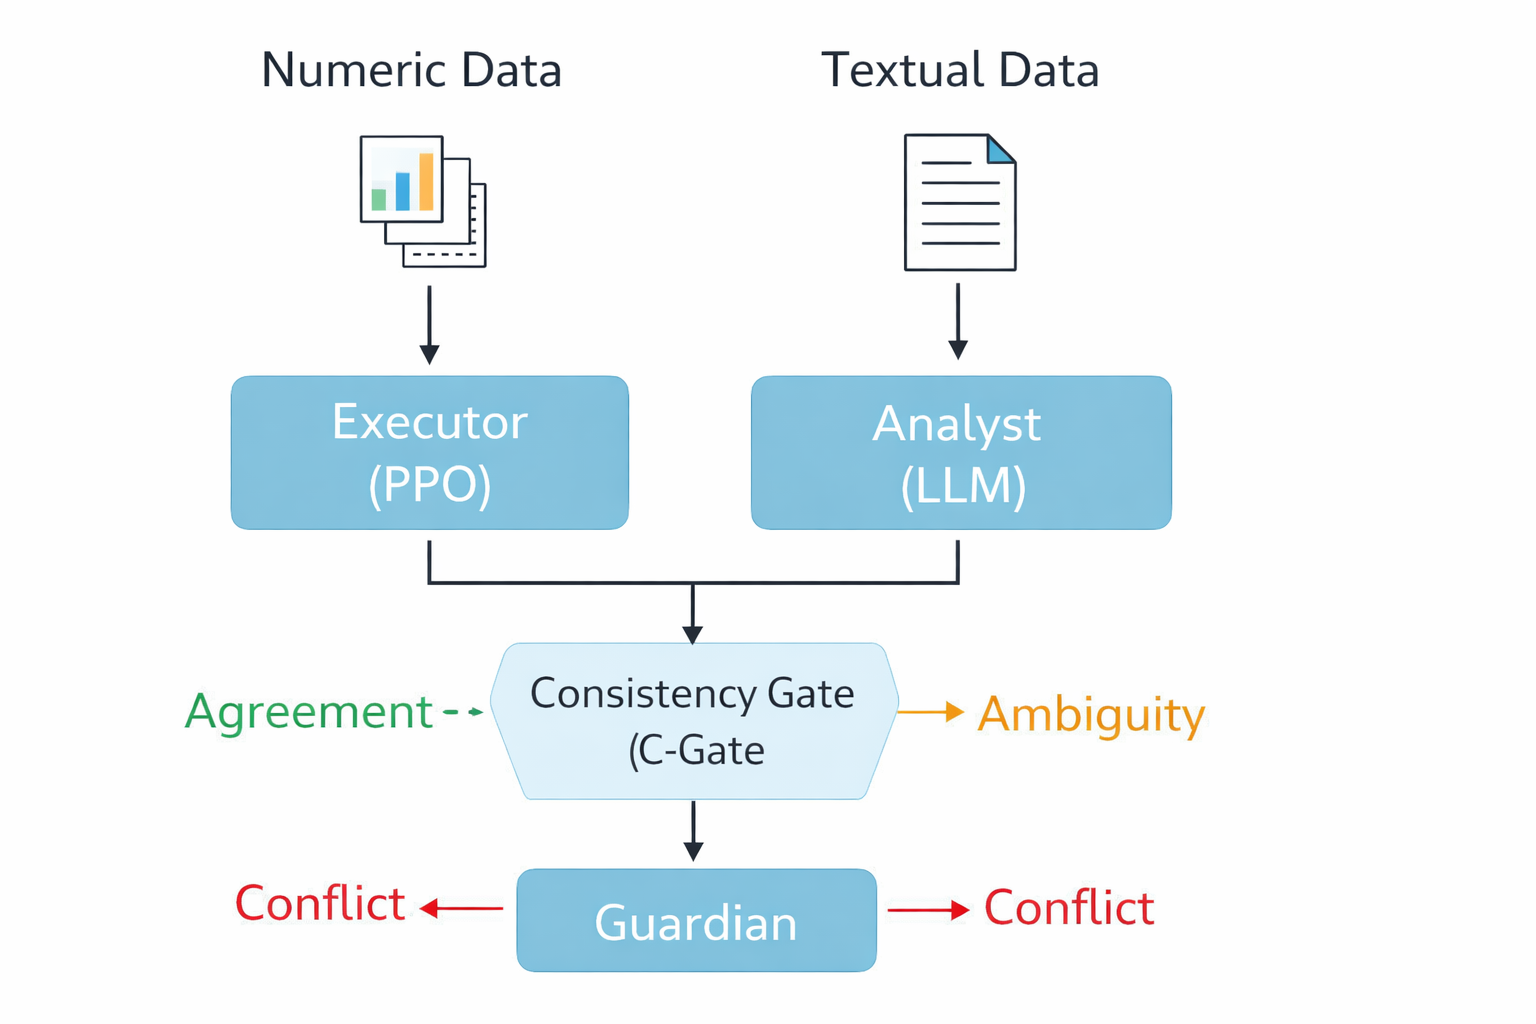
\includegraphics[width=\linewidth]{architecture.png}
  % \fbox{\parbox{0.9\textwidth}{\centering\vspace{4cm}
  %   \textit{Architecture diagram placeholder.}\\[0.5em]
  %   Two parallel input channels (numeric $\rightarrow$ Executor,
  %   text $\rightarrow$ Analyst) feeding into the C-Gate,
  %   which classifies the regime and forwards to the Guardian
  %   for final action selection.
  % \vspace{4cm}}}
  \caption{System architecture of the Robust Trinity. Market features feed
    the Executor (left channel) while news headlines feed the Analyst (right
    channel). The C-Gate computes a divergence score $\Delta_t$ from both
    agents' outputs and classifies the operating regime. The Guardian
    enforces hard constraints (Stage~1) and applies regime-dependent
    position sizing (Stage~2) before emitting the final trading action.}
  \label{fig:architecture}
\end{figure}


%--------------------------------------------------------------
\subsection{Formal Problem Formulation}
\label{sec:problem-formulation}
%--------------------------------------------------------------

The trading task is formulated as a sequential decision-making problem over a
discrete time horizon $t = 1, \ldots, T$, where each step corresponds to one
trading day. At each step the system observes a composite state
$\mathbf{O}_t = (s_t, x_t)$ comprising numeric market features
$s_t \in \mathbb{R}^{d}$ and a concurrent textual context
$x_t \in \mathcal{X}$ (a set of news headlines). The system produces a
final action $a_t \in \mathcal{A} = \{\text{flat}, \text{long},
\text{short}\}$---a position target rather than a trade order---from
which the environment computes the necessary trade.

The Executor is modelled as a Markov Decision Process
$(\mathcal{S}, \mathcal{A}, P, R, \gamma)$, where $\mathcal{S}$ denotes
the numeric observation space, $\mathcal{A} = \{0, 1, 2\}$ the
position-target action space, $P$ the (unknown) transition dynamics,
$R$ the reward function, and $\gamma = 0.95$ the discount factor. The
Executor's policy $\pi_\theta(a \mid s_t)$ is trained offline via PPO to
maximise expected discounted return
$\mathbb{E}\bigl[\sum_{t=0}^{T} \gamma^t\, r_t\bigr]$, where
$r_t = \log(1 + R_t^{\text{portfolio}})$ is the log-return reward.

The system's overall objective, however, differs from standard RL: rather
than learning a policy online, the goal is to produce safe, economically
viable actions from frozen components by detecting and containing
cross-modal inconsistencies---whether arising from natural market
non-stationarity or from adversarial manipulation of the input channels.


%--------------------------------------------------------------
\subsection{Threat Model}
\label{sec:threat-model}
%--------------------------------------------------------------

The system assumes an inference-time adversarial setting in which an external
actor may corrupt the inputs to either or both agent channels. Two attack
vectors are considered, matching the channel-independence structure of the
architecture:

\begin{description}
  \item[Analyst poisoning.] The adversary corrupts a fraction of the
    Analyst's directional signals by flipping buy recommendations to sell
    and vice versa ($d_{\mathrm{LLM}} \rightarrow \bar{d}_{\mathrm{LLM}}$),
    while leaving hold signals unchanged. This models an attacker who can
    manipulate the textual input channel---for instance, through headline
    fabrication or prompt injection---such that the LLM produces inverted
    directional advice.
  \item[Executor perturbation.] The adversary injects additive Gaussian
    noise into the Executor's numeric observations
    ($s_t \rightarrow s_t + \boldsymbol{\epsilon}$, where
    $\boldsymbol{\epsilon} \sim \mathcal{N}(\mathbf{0}, \sigma^2 \mathbf{I})$),
    modelling data-feed corruption, sensor noise, or adversarial
    perturbation of market features.
\end{description}

The adversary is assumed to have no access to internal model parameters and
cannot control both channels simultaneously. However, partial observability
and data inconsistencies may be exploited to degrade decision quality. The
adversary's objective is to induce erroneous actions that increase portfolio
drawdown. The C-Gate is designed to detect exactly this class of attack: when
one channel is corrupted, the divergence $\Delta_t$ rises, shifting the
system into the Ambiguity or Conflict regime and triggering the Guardian's
protective response.

%--------------------------------------------------------------
\subsection{The Executor (PPO Agent)}
\label{sec:executor}
%--------------------------------------------------------------

The Executor is a RL agent trained via (PPO)~\cite{schulman2017proximalpolicyoptimizationalgorithms}
to map numeric market observations to position targets. It operates
exclusively on structured price and volume data, with no access to textual
inputs, preserving the channel-independence invariant described in
Section~\ref{sec:architecture-overview}.

\paragraph{Trading environment.}
The Executor operates inside a custom Gymnasium-compatible environment. At
each daily timestep $t$, the agent selects an action
$a_t \in \{0, 1, 2\}$ representing a \emph{position target}---flat, long,
or short, respectively. The environment computes the trade required to reach
the target position from the current one and applies transaction costs of
15~basis points per unit of position change (10~bps brokerage commission plus
5~bps slippage). The slippage estimate is deliberately conservative for
AAPL, whose typical bid-ask spread is 1--3~bps, providing a safety margin
against the infinite-liquidity assumption inherent in backtesting.

\paragraph{Observation space.}
The observation vector is constructed by concatenating a lookback window of
$w = 10$ trading days of feature vectors with a three-dimensional portfolio
state, yielding $\mathbf{o}_t \in \mathbb{R}^{143}$ (i.e.,
$10 \times 14 + 3$). The 14 features, listed in
Table~\ref{tab:features}, are derived purely from OHLCV data.
All features are normalised using a rolling z-score with a 252-day window
(minimum 20 periods):
\begin{equation}
  z_{t,i} = \frac{x_{t,i} - \bar{x}_{i}^{(w)}}{\sigma_{i}^{(w)}},
\end{equation}
where $\bar{x}_{i}^{(w)}$ and $\sigma_{i}^{(w)}$ are the rolling mean and
standard deviation of feature $i$ over the preceding 252 trading days.
The three portfolio-state features appended to each observation are:
current position ($\{-1, 0, +1\}$), unrealised profit-and-loss (as a
fraction of portfolio value), and the number of days since the last trade.

% \begin{table}[t]
% \centering
% \caption{The 14 technical features comprising the Executor's numeric
%   observation channel. All are derived from OHLCV data and z-normalised
%   with a 252-day rolling window.}
% \label{tab:features}
% \begin{tabular}{@{}llp{7cm}@{}}
% \toprule
% \textbf{\#} & \textbf{Feature} & \textbf{Description} \\
% \midrule
% 1  & \texttt{log\_return}       & $\log(C_t / C_{t-1})$ \\
% 2  & \texttt{rsi}               & Relative Strength Index (14-day, Wilder's EMA) \\
% 3  & \texttt{macd\_line}        & MACD line (EMA$_{12}$ $-$ EMA$_{26}$) \\
% 4  & \texttt{macd\_signal}      & MACD signal line (EMA$_9$ of MACD line) \\
% 5  & \texttt{macd\_histogram}   & MACD line $-$ signal line \\
% 6  & \texttt{bb\_upper}         & Upper Bollinger Band (20-day, $2\sigma$) \\
% 7  & \texttt{bb\_lower}         & Lower Bollinger Band (20-day, $2\sigma$) \\
% 8  & \texttt{bb\_percent\_b}    & Bollinger \%B: $(C_t - \text{lower}) / (\text{upper} - \text{lower})$ \\
% 9  & \texttt{atr}               & Average True Range (14-day EMA) \\
% 10 & \texttt{volume\_ratio}     & Daily volume / 20-day SMA of volume \\
% 11 & \texttt{realized\_vol}     & Rolling 20-day standard deviation of log returns \\
% 12 & \texttt{close}             & Closing price (z-normalised, not raw) \\
% 13 & \texttt{high\_low\_range}  & $(H_t - L_t) / C_t$ \\
% 14 & \texttt{close\_open\_return} & $(C_t - O_t) / O_t$ \\
% \bottomrule
% \end{tabular}
% \end{table}

\paragraph{Reward function.}
The reward at each timestep is the log-return of the portfolio:
\begin{equation}
  r_t = \log\!\bigl(1 + R_t^{\text{portfolio}}\bigr),
\end{equation}
where $R_t^{\text{portfolio}}$ is the one-step portfolio return after
transaction costs. This reward is stateless and monotonically aligned with
economic performance. An alternative reward function---the Differential
Sharpe Ratio~\cite{moody2001learning}---was evaluated and abandoned, as
discussed in Section~\ref{sec:technical-alternatives}.

\paragraph{Training procedure.}
Training uses the Stable-Baselines3~\cite{raffin2021stable}
implementation of PPO with the hyperparameters listed in
Table~\ref{tab:ppo-hyperparams}. The policy network is a two-layer MLP
with 64 hidden units per layer and Tanh activations, with separate heads
for the policy ($\pi$) and value function ($V$). Eight parallel
environments are used for rollout collection. Reward normalisation via
\texttt{VecNormalize} is disabled (\texttt{norm\_reward=False}) to
preserve the log-return signal magnitude; observation normalisation is
likewise disabled (\texttt{norm\_obs=False}) because the features are
already z-normalised. Early stopping with patience 10 monitors validation
Sharpe ratio: training halts if no improvement is observed for 10
consecutive rollouts.

\begin{table}[t]
\centering
\caption{Frozen PPO hyperparameters. All values are from configuration v4,
  which was the only configuration to pass the policy-learning diagnostic
  (Section~\ref{sec:seed-selection}).}
\label{tab:ppo-hyperparams}
\begin{tabular}{@{}ll@{}}
\toprule
\textbf{Hyperparameter} & \textbf{Value} \\
\midrule
Learning rate            & $1.98 \times 10^{-4}$ \\
Discount factor $\gamma$ & 0.95 \\
Entropy coefficient      & 0.001 \\
Rollout steps (\texttt{n\_steps})  & 2{,}048 \\
Mini-batch size          & 64 \\
PPO epochs               & 10 \\
GAE $\lambda$            & 0.95 \\
Clip range               & 0.2 \\
Parallel environments    & 8 \\
Total timesteps          & 600{,}000 \\
Early-stopping patience  & 10 \\
Reward normalisation     & False \\
Reward type              & log-return \\
Policy architecture      & MLP $[64, 64]$, Tanh \\
\bottomrule
\end{tabular}
\end{table}

\paragraph{Seed selection and freezing.}
\label{sec:seed-selection}
Twenty seeds are trained under the configuration in
Table~\ref{tab:ppo-hyperparams}. To distinguish genuinely learned policies
from near-uniform ones whose \texttt{argmax} behaviour arises from
initialisation noise, a two-stage selection filter is applied:

\begin{enumerate}
  \item \textbf{Hard filter.} Any seed whose mean \emph{entropy ratio}
    (observed policy entropy divided by maximum entropy $\log 3$) exceeds
    0.90 across the test split is discarded. An entropy ratio above 0.90
    indicates a near-uniform distribution that has not learned meaningful
    directional preferences.
  \item \textbf{Ranking.} Surviving seeds are ranked by a combined score:
    $\text{val\_sharpe} + 0.5 \times \text{test\_sharpe}$. The 0.5 weight
    on test Sharpe penalises overfitting to the validation period while
    still rewarding generalisation.
\end{enumerate}

The top four seeds are frozen and stored with their model checkpoints and
normalisation statistics. Table~\ref{tab:frozen-seeds} lists the selected
seeds.

\begin{table}[t]
\centering
\caption{Frozen seeds selected from the v4 training run (20 candidates).
  All four pass the entropy-ratio hard filter ($< 0.90$).}
\label{tab:frozen-seeds}
\begin{tabular}{@{}ccccc@{}}
\toprule
\textbf{Seed} & \textbf{Entropy Ratio} & \textbf{Val Sharpe}
  & \textbf{Test Sharpe} & \textbf{Combined Score} \\
\midrule
123  & 0.321 & $+1.122$ & $-0.427$ & $+0.909$ \\
4444 & 0.299 & $+0.065$ & $-1.273$ & $-0.571$ \\
9999 & 0.831 & $-0.179$ & $-1.194$ & $-0.776$ \\
6789 & 0.429 & $-0.176$ & $-1.214$ & $-0.783$ \\
\bottomrule
\end{tabular}
\end{table}


%--------------------------------------------------------------
\subsection{The Analyst (LLM Agent)}
\label{sec:analyst}
%--------------------------------------------------------------

The Analyst is a large language model that processes financial news
headlines and produces a directional trading recommendation. It operates
exclusively on unstructured text, with no access to numeric market data,
preserving the channel-independence invariant.

\paragraph{Model and deployment.}
The Analyst uses GPT-5 accessed through the Azure
OpenAI API (\texttt{gpt-5-chat} deployment). Inference is performed at
temperature $0.0$ (greedy decoding) to ensure deterministic, reproducible
outputs. Three LLM backends were implemented---Azure OpenAI (GPT-5),
Anthropic Claude, and local Ollama (Llama~3.1 8B)---but only GPT-5
signals are used in the final system, as the Llama~3.1 backend produced
an unacceptably high hold rate (90.3\%) that provided insufficient
directional variation for the C-Gate.

\paragraph{Prompt design.}
The system prompt assigns the model the role of a ``highly decisive
quantitative financial analyst'' and enforces four rules: (1)~reasoning
must precede the decision (chain-of-thought); (2)~any headline with
material sentiment must yield a buy or sell signal, not hold;
(3)~hold is reserved strictly for neutral or irrelevant headlines; and
(4)~no numeric market data may be used. Five few-shot examples
(2~buy, 2~sell, 1~hold) are prepended to each request as conversation
history to calibrate the model's directional aggressiveness. The prompt
was iteratively refined to shift the signal distribution from 97.7\%
hold (original conservative prompt with GPT-5) to the final distribution
of 59.9\% hold, 22.3\% buy, and 17.7\% sell.

\paragraph{Output schema.}
Responses are constrained to a JSON schema enforced via a Pydantic model:
\begin{verbatim}
{"reasoning": "<chain-of-thought>",
 "decision": "<hold | buy | sell>"}
\end{verbatim}
The \texttt{reasoning} field is placed first in the schema to force the
model to articulate its analysis before committing to a decision---a
deliberate prompt-engineering choice, as LLMs that reason before deciding
tend to produce better-calibrated outputs~\cite{wei2022chain}. The
reasoning trace does not enter the divergence computation but is forwarded
to the Guardian during Conflict-regime timesteps for audit logging.
Notably, the schema contains \emph{no confidence score}: early
experiments with a $c \in [0,1]$ field showed poor calibration, and the
adopted divergence metric $\Delta_t$ (Section~\ref{sec:cgate}) does not
require one.

\paragraph{Precomputation and caching.}
All Analyst signals are precomputed offline and cached to a JSON file,
keyed by a deterministic SHA-256 hash of the tuple
$(\text{ticker}, \text{date}, \text{headline})$. This design enables
exact reproducibility regardless of future API changes, eliminates
inference latency from the evaluation loop, and controls costs (1{,}021
API calls for the full dataset). Atomic file writes (write to temporary
file, then rename) ensure cache integrity if the pipeline is interrupted
mid-run. The final signal file contains 1{,}021 entries covering 81.2\%
of trading days in the study period; days without a matching headline
receive no Analyst signal and are treated as $\Delta_t = 1.0$ (automatic
Conflict regime), which is safe by design.

%--------------------------------------------------------------
\subsection{The Consistency Gate (C-Gate)}
\label{sec:cgate}
%--------------------------------------------------------------

The C-Gate is the core coordination mechanism of the Robust
Trinity. It quantifies the divergence between the Executor's learned policy
and the Analyst's discrete recommendation, classifying each timestep into
one of three operating regimes that govern the Guardian's response.

\paragraph{Divergence metric.}
At each timestep $t$, the Executor produces a stochastic policy
$\pi_{\mathrm{RL}}(\cdot \mid s_t) \in \mathbb{R}^3$ over the three
position targets, and the Analyst produces a discrete decision
$d_{\mathrm{LLM}} \in \{\text{hold}, \text{buy}, \text{sell}\}$, mapped to
action indices $\{0, 1, 2\}$. The divergence is defined as:
\begin{equation}
\label{eq:delta}
  \Delta_t \;=\; 1 \;-\; \pi_{\mathrm{RL}}\!\bigl(d_{\mathrm{LLM}} \mid s_t\bigr),
\end{equation}
where $\pi_{\mathrm{RL}}(d_{\mathrm{LLM}} \mid s_t)$ is the probability
that the Executor's policy assigns to the Analyst's recommended action
given the current market state. This metric is bounded in $[0, 1]$:
$\Delta_t \approx 0$ when the Executor strongly agrees with the Analyst
(high probability mass on the recommended action), and
$\Delta_t \approx 1$ when the Executor assigns near-zero probability to
it (strong disagreement).

The metric is deliberately \emph{asymmetric}: it queries only the
Executor's probability for the Analyst's action, rather than comparing two
full distributions via a symmetric measure such as Jensen--Shannon
divergence. This design avoids the need for a pseudo-distribution from the
Analyst---which would require a calibrated confidence score that LLMs
cannot reliably provide (Section~\ref{sec:technical-alternatives})---and
ensures that $\Delta_t$ is fully determined by information already
available in the pipeline. The policy probabilities are computed at
temperature $T = 1.0$ (raw softmax over the policy network's logits),
preserving the continuous information in the learned distribution.

\paragraph{Three-regime classification.}
The divergence $\Delta_t$ is compared against two thresholds
$\tau_{\mathrm{low}}$ and $\tau_{\mathrm{high}}$ to classify the
operating regime:
\begin{equation}
\label{eq:regimes}
  \text{regime}_t =
  \begin{cases}
    \textsc{Agreement}  & \text{if } \Delta_t \leq \tau_{\mathrm{low}}, \\
    \textsc{Ambiguity}  & \text{if } \tau_{\mathrm{low}} < \Delta_t
                          \leq \tau_{\mathrm{high}}, \\
    \textsc{Conflict}   & \text{if } \Delta_t > \tau_{\mathrm{high}}.
  \end{cases}
\end{equation}

The three regimes govern execution as follows:
\begin{description}
  \item[Agreement] ($\Delta_t \leq \tau_{\mathrm{low}}$): The Executor and
    Analyst concur. Execute $\operatorname{argmax}(\pi_{\mathrm{RL}})$ at
    full position size (1.0) with no stop-loss.
  \item[Ambiguity] ($\tau_{\mathrm{low}} < \Delta_t \leq
    \tau_{\mathrm{high}}$): Partial disagreement. Execute
    $\operatorname{argmax}(\pi_{\mathrm{RL}})$ at reduced position size
    (0.5) with a 2\% stop-loss.
  \item[Conflict] ($\Delta_t > \tau_{\mathrm{high}}$): Strong
    disagreement. Override to flat (action$\,= 0$) and forward the
    Analyst's reasoning trace to the Guardian for audit logging.
\end{description}

This three-regime design enables \emph{graceful degradation}: rather than
a brittle binary switch between ``trust'' and ``reject,'' the system
transitions smoothly through an intermediate conservative posture. The
Ambiguity regime is particularly important---it allows trading to continue
under moderate uncertainty while limiting exposure through position scaling
and stop-losses.

\paragraph{Threshold calibration.}
\label{sec:calibration}
The thresholds $\tau_{\mathrm{low}}$ and $\tau_{\mathrm{high}}$ are
calibrated from the empirical distribution of $\Delta_t$ on the validation
split. Specifically, $\Delta_t$ values are collected across all four frozen
seeds on the validation period (452 observations in total) and the
thresholds are set to the 30th and 80th percentiles of this pooled
distribution:
\begin{equation}
  \tau_{\mathrm{low}} = P_{30}(\Delta_{\mathrm{val}}),
  \qquad
  \tau_{\mathrm{high}} = P_{80}(\Delta_{\mathrm{val}}).
\end{equation}
This data-driven approach produces $\tau_{\mathrm{low}} = 0.6935$ and
$\tau_{\mathrm{high}} = 0.9877$, yielding a regime distribution of
approximately 30\% Agreement, 50\% Ambiguity, and 20\% Conflict on the
validation set. The percentile choice (30/80) was informed by a sweep over
candidate pairs; the key constraint is that the Conflict regime should
capture roughly the top quintile of $\Delta_t$ values, corresponding to
the most extreme disagreements.

\paragraph{Missing-headline handling.}
On trading days without a matching Polygon.io headline, no Analyst signal
is available. These days are assigned $\Delta_t = 1.0$, which places them
unconditionally in the Conflict regime (fail-safe to flat). This is a
conservative default: the system declines to trade when one information
channel is absent, rather than relying solely on the Executor.


%--------------------------------------------------------------
\subsection{The Guardian}
\label{sec:guardian}
%--------------------------------------------------------------

The Guardian is a rule-based risk management module that operates in two
sequential stages. Stage~1 enforces unconditional hard constraints that
fire before the C-Gate, while Stage~2 applies regime-dependent position
sizing and risk controls after the C-Gate has classified the operating
regime.

\paragraph{Stage 1: Hard constraints.}
Stage~1 evaluates four portfolio-level constraints against the current
portfolio state. If \emph{any} constraint is violated, the proposed action
is overridden to flat (action$\,= 0$) regardless of the C-Gate's
output---Stage~2 is not invoked. The four constraints are:

\begin{enumerate}
  \item \textbf{Daily loss circuit breaker.} If the day's cumulative loss
    exceeds 5\% of portfolio value, all non-flat actions are blocked.
  \item \textbf{Drawdown circuit breaker.} If the portfolio's drawdown
    from its historical peak exceeds 15\%, all non-flat actions are
    blocked.
  \item \textbf{Position size limit.} If the current absolute position
    already equals the maximum allowed (100\% of portfolio value), no
    further directional trades are permitted.
  \item \textbf{Cash reserve.} Long entries are blocked if cash falls
    below 10\% of portfolio value.
\end{enumerate}

These thresholds are configured in \texttt{configs/guardian.yaml} and
summarised in Table~\ref{tab:guardian-config}.

\begin{table}[t]
\centering
\caption{Guardian configuration parameters.}
\label{tab:guardian-config}
\begin{tabular}{@{}llll@{}}
\toprule
\textbf{Stage} & \textbf{Parameter} & \textbf{Value} & \textbf{Effect} \\
\midrule
\multirow{4}{*}{Stage 1}
  & \texttt{max\_daily\_loss}     & 0.05  & 5\% daily loss $\rightarrow$ halt \\
  & \texttt{max\_drawdown}        & 0.15  & 15\% drawdown $\rightarrow$ halt \\
  & \texttt{max\_position\_size}  & 1.0   & No leverage \\
  & \texttt{min\_cash\_reserve}   & 0.10  & 10\% cash floor \\
\midrule
\multirow{3}{*}{Stage 2}
  & \texttt{ambiguity\_position\_scale} & 0.5  & Half-size in Ambiguity \\
  & \texttt{ambiguity\_stop\_loss}      & 0.02 & 2\% stop-loss in Ambiguity \\
  & \texttt{conflict\_action}           & 0    & Flat in Conflict \\
\bottomrule
\end{tabular}
\end{table}

\paragraph{Stage 2: Adaptive policy.}
If Stage~1 allows the proposed action, Stage~2 applies regime-dependent
adjustments based on the C-Gate's classification:

\begin{description}
  \item[Agreement regime.] The action passes through at full position size
    (scale$\,= 1.0$) with no stop-loss override. This is the system's
    normal operating mode.
  \item[Ambiguity regime.] The action is preserved but the position is
    scaled to 50\% and a 2\% stop-loss is imposed. This halves the
    maximum per-step loss on ambiguous days, providing a mechanical
    drawdown buffer.
  \item[Conflict regime.] The action is overridden to flat
    (action$\,= 0$, scale$\,= 0.0$). The Analyst's reasoning trace is
    logged for post-hoc audit but does not influence the decision.
\end{description}

The two-stage design ensures that hard safety limits always take precedence
over regime-based modulation. In practice, Stage~1 circuit breakers fire
on 2--10\% of timesteps across the evaluation period---they are rare
emergency overrides, not routine interventions.


%--------------------------------------------------------------
\subsection{Decision Step Workflow}
\label{sec:decision-workflow}
%--------------------------------------------------------------

At each trading day $t$, the system executes the following steps:

\begin{enumerate}
  \item \textbf{Parallel signal generation.}
    The Executor receives the numeric observation $\mathbf{o}_t$ and
    produces a policy distribution
    $\pi_{\mathrm{RL}}(\cdot \mid s_t) \in \mathbb{R}^3$. Independently,
    the Analyst's precomputed signal for date $t$ is loaded from cache,
    yielding $(d_{\mathrm{LLM}},\, r_{\mathrm{LLM}})$. The two channels
    share no information.

  \item \textbf{Guardian Stage~1 (hard constraints).}
    The current portfolio state---value, peak, drawdown, daily PnL, cash
    position---is evaluated against the four hard constraints
    (Table~\ref{tab:guardian-config}). If any constraint is violated, the
    action is overridden to flat and the pipeline short-circuits; Steps~3
    and~4 are skipped.

  \item \textbf{C-Gate divergence and regime classification.}
    The divergence
    $\Delta_t = 1 - \pi_{\mathrm{RL}}(d_{\mathrm{LLM}} \mid s_t)$
    is computed and compared against the calibrated thresholds
    $\tau_{\mathrm{low}}$ and $\tau_{\mathrm{high}}$ to classify the
    regime as Agreement, Ambiguity, or Conflict
    (Equation~\ref{eq:regimes}). The candidate action is set to
    $\operatorname{argmax}(\pi_{\mathrm{RL}})$ in the Agreement and
    Ambiguity regimes, or to flat in the Conflict regime.

  \item \textbf{Guardian Stage~2 (adaptive policy).}
    The regime classification determines position sizing: full size in
    Agreement, half size with 2\% stop-loss in Ambiguity, zero size in
    Conflict. In the Conflict regime, the Analyst's reasoning trace
    $r_{\mathrm{LLM}}$ is logged for audit.

  \item \textbf{Execution.}
    The final action and position scale are applied: the environment
    computes the trade required to reach the target position from the
    current one, applies transaction costs, and updates the portfolio
    state for the next timestep.
\end{enumerate}

If no headline is available for date $t$, Step~1 sets
$\Delta_t = 1.0$, which routes directly to Conflict in Step~3.
All intermediate values---$\pi_{\mathrm{RL}}$, $d_{\mathrm{LLM}}$,
$\Delta_t$, regime, Stage~1 violations, and the final action---are logged
per timestep for post-hoc analysis.

%--------------------------------------------------------------
\subsection{Evaluation Setup}
\label{sec:evaluation-setup}
%--------------------------------------------------------------

Following the DSR framework ~\cite {johannesson2014design}, the artefact is
evaluated to assess how well it satisfies the defined requirements of
adversarial robustness and financial safety. Evaluation is conducted
through historical backtesting with post-hoc adversarial injection on the
test split. There is no separate simulation environment; all experiments
use the same AAPL daily-bar dataset described in
Section~\ref{sec:data_collection}.

\paragraph{Data splits.}
The dataset is partitioned into four non-overlapping periods, listed in
Table~\ref{tab:data_splits}. The warmup period provides history for rolling
indicators but is never used for training, validation, or testing. The
training period is used to train the Executor's PPO policy. The validation
period is used for early stopping, C-Gate threshold calibration, and seed
selection. The test period is held out for all reported results.

% \begin{table}[t]
% \centering
% \caption{Chronological data splits. No overlap exists between any two
%   periods.}
% \label{tab:splits}
% \begin{tabular}{@{}llr@{}}
% \toprule
% \textbf{Split} & \textbf{Date Range} & \textbf{Trading Days} \\
% \midrule
% Warmup     & 2020-01-01 -- 2020-12-31 & 253 \\
% Train      & 2021-01-01 -- 2023-12-31 & 756 \\
% Validation & 2024-01-01 -- 2024-06-30 & 124 \\
% Test       & 2024-07-01 -- 2024-12-31 & 127 \\
% \bottomrule
% \end{tabular}
% \end{table}

\paragraph{System configurations.}
Five configurations are evaluated, forming a systematic ablation study in
which each variant removes one component to isolate its contribution:

\begin{enumerate}
  \item \textbf{Trinity} (full system): Executor + Analyst + C-Gate +
    Guardian. The complete architecture as described in
    Sections~\ref{sec:executor}--\ref{sec:decision-workflow}.
  \item \textbf{Executor-Only}: PPO $\operatorname{argmax}$ at full
    position size. No C-Gate, no Guardian, no Analyst. Isolates the raw
    RL policy.
  \item \textbf{Analyst-Only}: GPT-5 signals executed directly as
    position targets (buy$\,\rightarrow\,$long,
    sell$\,\rightarrow\,$short, hold$\,\rightarrow\,$flat) at full
    position size. No seed variation---a single deterministic run per
    split. Isolates the LLM's directional skill.
  \item \textbf{Trinity-no-CGate}: A naive agreement heuristic. If
    $\operatorname{argmax}(\pi_{\mathrm{RL}}) = d_{\mathrm{LLM}}$,
    execute at full position; otherwise execute
    $\operatorname{argmax}(\pi_{\mathrm{RL}})$ at half position. No
    $\Delta_t$ computation, no temperature scaling, no Guardian. Tests
    whether a simple agreement check captures most of the C-Gate's value.
  \item \textbf{Buy-and-Hold}: A passive benchmark that enters a long
    position on the first day and holds throughout the test period. Serves
    as a market-return reference.
\end{enumerate}

All seed-dependent configurations (Trinity, Executor-Only,
Trinity-no-CGate) are run across the four frozen seeds (123, 4444, 9999,
6789) and results are reported as both per-seed and mean$\,\pm\,$standard
deviation across seeds. The Analyst-Only and Buy-and-Hold baselines are
deterministic and produce a single run each.

\paragraph{Adversarial protocol.}
Robustness is evaluated under two attack vectors, matching the threat
model in Section~\ref{sec:threat-model}:

\begin{description}
  \item[Analyst poisoning.] A fraction $\rho \in \{0.10, 0.20, 0.30,
    0.40, 0.50\}$ of directional signals (buy and sell) are randomly
    selected and flipped (buy$\,\rightarrow\,$sell,
    sell$\,\rightarrow\,$buy); hold signals are unchanged. A fixed
    corruption seed (42) ensures reproducibility. The number of flipped
    signals ranges from 40 ($\rho = 0.10$) to 204 ($\rho = 0.50$) out of
    approximately 408 total directional signals in the test period.
  \item[Executor perturbation.] Additive Gaussian noise
    $\boldsymbol{\epsilon} \sim \mathcal{N}(\mathbf{0},\,
    \sigma^2 \mathbf{I})$ is injected into the Executor's observation
    vector at $\sigma \in \{0.10, 0.20, 0.30, 0.40, 0.50\}$. The noise
    is applied after z-normalisation, so $\sigma = 0.50$ represents half
    a standard deviation of perturbation on each feature.
\end{description}

Each attack is applied independently to all four system configurations
(Trinity, Executor-Only, Analyst-Only, Trinity-no-CGate) across all four
seeds, producing a total of $2 \times 5 \times 4 \times 4 = 160$
adversarial runs plus the Analyst-Only variants.

\paragraph{Metrics.}
Performance is assessed using the financial metrics defined in
Section~\ref{sec:financial-metrics}: annualised Sharpe ratio, Sortino
ratio, MaxDD, and total return. The primary robustness
indicator is the \emph{stability} of MaxDD under attack: a
robust system should exhibit a narrow MaxDD range across clean and
adversarial conditions, whereas a brittle system shows large MaxDD
increases under corruption. All metrics are computed on the test split;
validation-period results are reported only for calibration and diagnostic
purposes.

\paragraph{Statistical reporting.}
Results across the four seeds are summarised as mean$\,\pm\,$standard
deviation. No formal inferential tests (e.g., paired $t$-tests or
bootstrap confidence intervals) are applied, because four seeds provide
insufficient statistical power for such tests. This limitation is
acknowledged explicitly; the evaluation instead relies on consistent
directional patterns across seeds and attack levels to support its
conclusions.


%--------------------------------------------------------------
\subsection{Software Tools}
\label{sec:software-tools}
%--------------------------------------------------------------

Table~\ref{tab:software-tools} summarises the software tools used for
data collection, artefact development, evaluation, and thesis writing.

\begin{table}[t]
\centering
\caption{Software tools used in this thesis.}
\label{tab:software-tools}
\begin{tabular}{@{}lll@{}}
\toprule
\textbf{Purpose} & \textbf{Tool} & \textbf{Role} \\
\midrule
RL training       & Stable-Baselines3~\citep{raffin2021stable} / PyTorch
                  & PPO policy training and inference \\
Trading environment & Gymnasium (OpenAI)
                  & Custom \texttt{TradingEnv} wrapper \\
LLM inference     & Azure OpenAI API (GPT-5)
                  & Analyst signal generation \\
Market data       & Yahoo Finance (\texttt{yfinance})
                  & OHLCV download \\
News data         & Polygon.io REST API
                  & Headline collection \\
Feature engineering & NumPy, Pandas
                  & Technical indicators and z-normalisation \\
Data visualisation & Matplotlib, Seaborn
                  & Charts and figures \\
Experiment tracking & Weights \& Biases
                  & Hyperparameter sweeps and run logging \\
Configuration     & PyYAML, Pydantic
                  & Config files and schema validation \\
Version control   & Git / GitHub
                  & Code and experiment management \\
Document preparation & \LaTeX{} (Overleaf)
                  & Thesis typesetting \\
AI writing aid    & ChatGPT, Claude
                  & Proofreading and paraphrasing \\
\bottomrule
\end{tabular}
\end{table}

GPT-5 serves a dual role in this study: as the Analyst component within
the artefact and as a general-purpose research tool. Its use as a system
component is integral to the architecture and is evaluated through the
C-Gate mechanism. Separately, general-purpose LLMs (ChatGPT and Claude)
were used during the thesis writing process for proofreading, paraphrasing,
and brainstorming; all AI-assisted text was subsequently reviewed, verified,
and revised by the author. The specific use and impact of these tools is
further discussed in the Conclusions chapter.

%--------------------------------------------------------------
\section{Summary of Methodological Choices}
\label{sec:method-summary}
%--------------------------------------------------------------

Table~\ref{tab:method-summary} consolidates the key methodological choices
made throughout this chapter, linking each to its justification and the
section where it is discussed.

\begin{table}[ht]
\centering
\caption{Summary of methodological choices.}
\label{tab:method-summary}
\small
\begin{tabular}{@{}p{3.2cm}p{4.5cm}p{5.8cm}@{}}
\toprule
\textbf{Aspect} & \textbf{Choice} & \textbf{Justification} \\
\midrule
Research strategy
  & Design science research~\cite{johannesson2014design}
  & Artefact-centric goal; iterative multi-component design
    (Section~\ref{sec:research-strategy}) \\[4pt]

Market data
  & AAPL daily bars, Yahoo Finance
  & High liquidity, dense news coverage; single-ticker scope is a
    deliberate delimitation
    (Section~\ref{sec:data-collection}) \\[4pt]

News data
  & Polygon.io headlines, deduplicated
  & Professionally curated, daily cadence, no PII
    (Section~\ref{sec:data-collection}) \\[4pt]

LLM signals
  & GPT-5 via Azure OpenAI, precomputed offline
  & Strongest directional signal distribution (40.1\% directional);
    cached for reproducibility
    (Section~\ref{sec:analyst}) \\[4pt]

Divergence metric
  & $\Delta_t = 1 - \pi_{\mathrm{RL}}(d_{\mathrm{LLM}})$
  & Requires no confidence score from Analyst; fully determined by
    Executor's policy
    (Section~\ref{sec:cgate}) \\[4pt]

Temperature
  & $T = 1.0$ (raw policy probabilities)
  & Low temperatures collapse $\Delta$ to bimodal; $T=1.0$ preserves
    continuous spread
    (Section~\ref{sec:technical-alternatives}) \\[4pt]

Threshold calibration
  & Percentile-based ($p_{30}$/$p_{80}$) on validation $\Delta$
  & Data-driven; yields $\tau_{\mathrm{low}} = 0.6935$,
    $\tau_{\mathrm{high}} = 0.9877$
    (Section~\ref{sec:calibration}) \\[4pt]

Reward function
  & Log-return: $r_t = \log(1 + R_t^{\text{portfolio}})$
  & DSR signal too weak for PPO on 756 training days
    (Section~\ref{sec:technical-alternatives}) \\[4pt]

Policy architecture
  & MLP $[64, 64]$, Tanh
  & Larger networks (2$\times$128 ReLU) degraded policy learning
    (Section~\ref{sec:technical-alternatives}) \\[4pt]

Seed selection
  & Entropy ratio $< 0.90$, then combined score
  & Filters out near-uniform policies; 4 seeds frozen
    (Section~\ref{sec:seed-selection}) \\[4pt]

Risk management
  & Two-stage Guardian (hard constraints + adaptive policy)
  & Stage~1 enforces unconditional safety; Stage~2 modulates position
    sizing by regime
    (Section~\ref{sec:guardian}) \\[4pt]

Adversarial protocol
  & Post-hoc signal poisoning + observation noise
  & Targeted, reproducible; avoids simulator-fidelity confound
    (Section~\ref{sec:evaluation-setup}) \\[4pt]

Statistical reporting
  & Descriptive (mean $\pm$ std across 4 seeds)
  & Four seeds insufficient for formal inference; acknowledged as
    limitation
    (Section~\ref{sec:evaluation-setup}) \\
\bottomrule
\end{tabular}
\end{table}

% \subsubsection{System Architecture and Workflow}

% The Robust Trinity processes inputs through two parallel channels and one sequential arbitration layer. Market data (price, volume, order-book features) feeds the Optimiser, while unstructured text (news, filings, social media) feeds the Analyst. Both channels produce structured action signals---$a_{\mathrm{RL}}$ and $a_{\mathrm{LLM}}$, respectively---independently and in parallel, ensuring that neither modality conditions on the other's output before arbitration.

% These raw signals first pass through a hard-constraint filter (Guardian Stage~1), which unconditionally rejects actions that violate regulatory or position-limit boundaries. The surviving signals then enter the Consistency Gate, which computes a cross-modal divergence score $\Delta(a_{\mathrm{RL}}, a_{\mathrm{LLM}})$. This score, together with the candidate actions, is forwarded to the Guardian's adaptive stage (Stage~2), which selects the execution policy.

% Under low $\Delta$, the system executes normally under standard risk constraints; under moderate $\Delta$, it activates a conservative posture with reduced position sizes and tightened stop-losses; under high $\Delta$, it halts execution entirely and defaults to the Guardian's fail-safe policy. The final action emitted is therefore a function of both modality-specific reasoning and system-level consistency.

% \subsubsection{The Analyst (LLM-Based Agent)}

% We use Claude~4.5 (Sonnet variant) in the role of Analyst. This model demonstrates competitive performance on instruction-following and safety benchmarks~\cite{mazeika2024harmbenchstandardizedevaluationframework}, though adversarial robustness in the financial domain is ultimately ensured by the C-Gate mechanism rather than by any property of the LLM itself. Inputs to the Analyst include financial news headlines, social sentiment from Reddit/X, and corporate disclosures such as 10-K/10-Q snippets and earnings call transcripts. LLMs can provide reasoning to justify the proposed action and generalise across market contexts.

% To optimise the LLM's performance, we employ prompting strategies such as: (1)~chain-of-thought prompting to guide structured reasoning and ensure robust interpretation of unstructured inputs; (2)~role-playing prompts to simulate a financial analyst persona, enabling nuanced semantic processing and consistent signal generation; and (3)~few-shot examples to calibrate generalisation, yielding reliable action signals across diverse market contexts~\cite{NEURIPS2022_9d560961, NEURIPS2020_1457c0d6}.

% The Analyst outputs a structured signal $a_{\mathrm{LLM}} = (d, c, r)$, where $d \in \{\text{hold}, \text{buy}, \text{sell}\}$ is a directional recommendation, $c \in [0,1]$ is a confidence score, and $r$ is a chain-of-thought reasoning trace. This output is enforced via structured prompting that constrains responses to a fixed JSON schema, ensuring compatibility with the Optimiser's action space.

% \subsubsection{The Optimiser (RL-Based Agent)}

% The Optimiser learns a stochastic policy $\pi(a \mid s)$ that maps market state observations to trading actions---discrete allocations over $\{\text{hold}, \text{buy}, \text{sell}\}$. The state vector $s$ comprises price returns, order-book depth, realised volatility, and cross-asset correlation features, deliberately excluding any text-derived inputs to preserve channel independence from the Analyst. The learning objective maximises expected cumulative discounted reward
% \begin{equation}
% \mathbb{E}\left[\sum_{t=0}^{T} \gamma^t r_t\right],
% \end{equation}
% where $r_t$ encodes risk-adjusted portfolio return penalised by drawdown exposure.

% We adopt Proximal Policy Optimisation (PPO) as the training algorithm. PPO's clipped surrogate objective constrains policy updates to a trust region, providing stable convergence under the non-stationary reward distributions characteristic of financial time series~\cite{schulman2017proximalpolicyoptimizationalgorithms, 10.1145/3490354.3494366}. The Optimiser is pre-trained offline on historical and simulated market data, then deployed with a frozen policy within the Trinity. This is a deliberate architectural requirement: the C-Gate depends on a stable, competent $a_{\mathrm{RL}}$ signal to produce meaningful divergence scores. An agent still exploring would generate noise indistinguishable from adversarial inconsistency, undermining the fault model. Regime adaptation is handled through periodic offline retraining and validation rather than online learning during inference.

% \subsubsection{The Guardian (Rule-Based Risk Module)}

% Complementing the Analyst and Optimiser, the Guardian implements rule-based risk management in two stages. Outputs from both the Analyst and Optimiser are first passed through Guardian Stage~1, which filters out clearly illegal actions, such as those exceeding position limits or involving restricted securities. Guardian Stage~2 validates consistency between the Analyst and Optimiser. If the consistency metric $\Delta$ exceeds a threshold, execution is halted or shifted to a conservative mode (e.g., reduced leverage or defaulting to \textit{hold}); otherwise, the trade proceeds normally. The Guardian enhances robustness by enforcing strict rule-based compliance, preventing catastrophic failure~\cite{kirilenko2017flash, easley2011} in a critical domain such as financial trading.

% \subsubsection{The Consistency Gate (C-Gate)}

% We present the Consistency Gate (C-Gate), the core contribution of this study, which measures agreement between the Analyst and Optimiser. The Analyst output $a_{\mathrm{LLM}} = (d,c,r)$ is mapped to a pseudo-distribution over $\{\text{hold}, \text{buy}, \text{sell}\}$. For example, if $d=\text{buy}$ and $c=0.85$:
% \begin{equation}
% \hat{\pi}_{\mathrm{LLM}} = \left(\frac{1-c}{2},\; c,\; \frac{1-c}{2}\right) = (0.075,\,0.85,\,0.075).
% \end{equation}
% The remaining probability mass $1-c$ is distributed uniformly across non-selected actions. The divergence is defined as:
% \begin{equation}
% \Delta_t = \mathrm{JSD}\left(\hat{\pi}_{\mathrm{LLM}}, \pi_{\mathrm{RL}}\right),
% \end{equation}
% where Jensen--Shannon Divergence (JSD) is symmetric and bounded in $[0,1]$~\cite{61115}. Low $\Delta_t$ indicates agreement, while high $\Delta_t$ signals potential adversarial inconsistency.

% The C-Gate computes $\Delta(a_{\mathrm{RL}}, a_{\mathrm{LLM}})$ over the $(d, c)$ components only. The reasoning trace $r$ does not enter the divergence computation but is forwarded to the Guardian as interpretive context during high-$\Delta$ arbitration and logged for post-hoc audit, thereby providing an explainability layer that the Optimiser's learned policy cannot supply.

% The divergence governs a three-regime decision policy:
% \begin{itemize}
% \item $\Delta_t \leq \tau_{\text{low}}$ (Agreement): execution under standard constraints.
% \item $\tau_{\text{low}} < \Delta_t \leq \tau_{\text{high}}$ (Ambiguity): conservative mode with reduced exposure and tightened risk controls.
% \item $\Delta_t > \tau_{\text{high}}$ (Conflict): execution halt and fallback to fail-safe policy.
% \end{itemize}
% The thresholds $\tau_{\text{low}}$ and $\tau_{\text{high}}$ are calibrated empirically under benign and adversarial conditions, enabling smooth degradation rather than brittle binary switching.

% \subsubsection{Decision Step Workflow}

% At each decision step $t$, the Trinity executes the following workflow. The Optimiser receives state $s_t$, while the Analyst receives text input $x_t$. Both operate independently: the Optimiser outputs $\pi_{\mathrm{RL}}(\cdot \mid s_t)$, and the Analyst outputs $a_{\mathrm{LLM}}=(d,c,r)$. After passing Guardian Stage~1, the C-Gate computes:
% \begin{equation}
% \Delta_t = \mathrm{JSD}\left(\hat{\pi}_{\mathrm{LLM}}, \pi_{\mathrm{RL}}\right),
% \end{equation}
% and applies the three-regime policy to determine execution. All outputs, including $\Delta_t$ and $r$, are logged for audit.

% %--------------------------------------------------------------
% \subsection{Evaluation Setup} \label{sec:evaluation_setup}
% %--------------------------------------------------------------

% Following the DSR framework ~\cite{johannesson2014design}, the artifact is evaluated to assess how well it satisfies the defined requirements of adversarial robustness and financial performance. The evaluation is conducted in two complementary settings, corresponding to the data collection methods described in Section~\ref{sec:data_collection}.

% \textbf{Setting~1: Adversarial simulation.} Using ABIDES~\cite{10.1145/3384441.3395986}, adversarial agents are introduced that manipulate numeric and semantic inputs. Attack intensity is systematically varied across low, moderate, and severe levels to assess how robustness degrades under increasing adversarial pressure. This controlled experimental setup enables isolation of the effects of individual attack vectors (numeric perturbation, semantic manipulation, or both) on system behaviour.

% \textbf{Setting~2: Historical backtesting.} The system is backtested on Nasdaq-100 data (January~2023--December~2024) under benign conditions to validate that the architecture achieves competitive financial performance in the absence of adversarial manipulation.

% \textbf{Baselines and ablation.} We compare the full Robust Trinity against three baselines: (1)~Optimiser-only, (2)~Analyst-only, and (3)~Trinity without C-Gate. All share identical Guardian constraints. The baselines form a systematic ablation study: each removes one component---semantic reasoning, numeric reasoning, or divergence-based arbitration---isolating its contribution to overall performance and robustness. A degradation in robustness without the C-Gate, while benign performance remains stable, validates the thesis that cross-modal arbitration provides resilience beyond individual components.

% \textbf{Metrics.} Performance is assessed using financial metrics (PnL, Sharpe ratio, maximum drawdown, Value-at-Risk, Expected Shortfall) and robustness metrics (performance degradation and action stability). Descriptive statistics (means, standard deviations) and, where applicable, statistical significance tests are used to compare configurations. These evaluations test whether structural fault tolerance limits adversarial impact.

% %--------------------------------------------------------------
% \subsection{Software Tools} \label{sec:software_tools}
% %--------------------------------------------------------------

% Table~\ref{tab:software_tools} summarises the software tools used for data collection, analysis, artifact development, and AI-based content generation in this thesis.

% \begin{table}[h]
% \centering
% \caption{Software tools used in the thesis.}
% \label{tab:software_tools}
% \begin{tabular}{@{}lll@{}}
% \toprule
% \textbf{Purpose} & \textbf{Tool} & \textbf{Role} \\
% \midrule
% Market simulation & ABIDES~\cite{10.1145/3384441.3395986} & Adversarial data generation \\
% RL training & Stable-Baselines3 / PyTorch & PPO policy training \\
% LLM inference & Claude~4.5 Sonnet (Anthropic API) & Analyst agent \\
% Statistical analysis & Python (NumPy, Pandas, SciPy) & Metric computation \\
% Data visualisation & Matplotlib / Seaborn & Charts and figures \\
% Backtesting framework & Custom Python pipeline & Historical evaluation \\
% AI-based writing aid & ChatGPT / Claude & Proofreading, paraphrasing \\
% Version control & Git / GitHub & Code and manuscript management \\
% \bottomrule
% \end{tabular}
% \end{table}

% Of particular note regarding AI-based tools: Claude~4.5 Sonnet serves a dual role---as the Analyst component within the artifact and as a research tool. Its use as a system component is integral to the architecture and is evaluated through the C-Gate mechanism. Separately, general-purpose LLMs (ChatGPT and Claude) were used during the thesis writing process for proofreading, paraphrasing, and brainstorming; all AI-assisted text was subsequently reviewed, verified, and revised by the authors. The specific use and impact of these tools is further discussed in the Conclusions chapter.

% %--------------------------------------------------------------
% \section{Summary of Methodological Choices} \label{sec:method_summary}
% %--------------------------------------------------------------

% Table~\ref{tab:method_summary} provides an overview of the methodological choices made in this thesis and their justification.

% \begin{table}[h]
% \centering
% \caption{Summary of research strategy and methods.}
% \label{tab:method_summary}
% \begin{tabular}{@{}p{3.5cm}p{4cm}p{5.5cm}@{}}
% \toprule
% \textbf{Aspect} & \textbf{Choice} & \textbf{Justification} \\
% \midrule
% Research strategy & Design science research~\cite{johannesson2014design} & Thesis develops and evaluates an artifact (Robust Trinity) \\
% DSR framework & Johannesson \& Perjons~\cite{johannesson2014design} & Provides structured activities for artifact-centred research \\
% Evaluation strategy & Experiment (simulation + backtest) & Enables controlled adversarial manipulation \\
% Data collection & Simulation (ABIDES) + historical data & Combines controlled and realistic settings \\
% Data analysis & Quantitative (financial + robustness metrics) & Aligns with measurable research question \\
% \bottomrule
% \end{tabular}
% \end{table}
